\section{Sprint 3}%Corrección de issues 

\subsection{Planificación}
\begin{itemize}
    \item \textbf{Inicio}: 7 de julio del 2015.
    \item \textbf{Fin}: 16 de agosto del 2015.
\end{itemize}

\begin{figure}[h!]
  \centering
  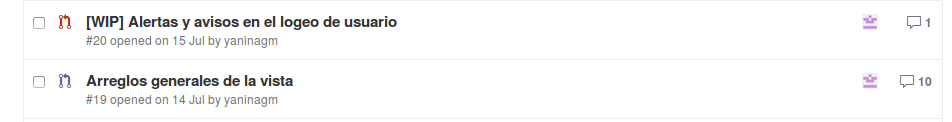
\includegraphics[width=.8\textwidth]{img/3-PR_1_front}
  \caption{Pull request realizados en el sprint  3}
  \label{pull_request_sprint_3}
\end{figure}
\begin{figure}[h!]
  \centering
  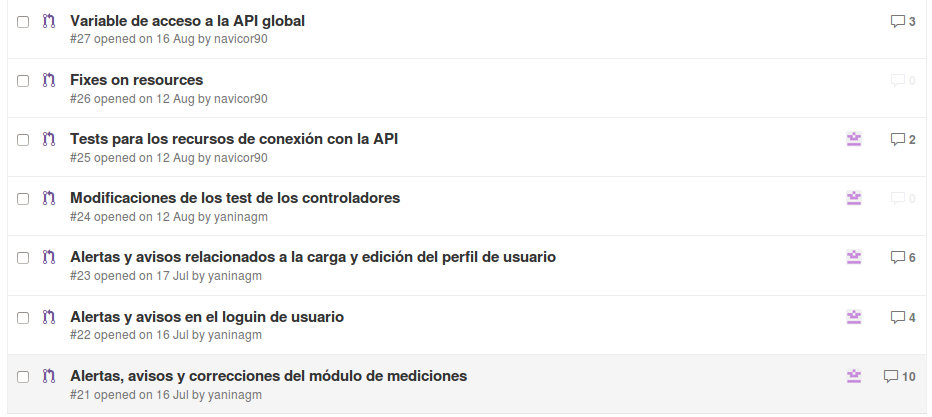
\includegraphics[width=.8\textwidth]{img/3-PR_2_front}
  \caption{Pull request realizados en el sprint  3}
  \label{3-PR_back}
\end{figure}

	{\scriptsize
	\begin{center} %sidewaystable
	\centering
	%\begin{adjustbox}{max width=\textheight}
    \resizebox{\textwidth}{!}
    {
	\begin{tabular}{|l|l|p{5cm}|l|l|}
	    \hline
	        \textbf{Área a cargo} &
	        \textbf{Responsable} &        
	        \textbf{Tarea} &
	        \textbf{US} &
            \textbf{Tiempo}\\
   		\hline
       
	    Documentación& Michael Manganiello & Trabajo práctico integrador nº2 ``Planificación de proyectos informáticos''. & & 17 horas \\ \hline
        Documentación & Iván Terreno & Trabajo práctico integrador nº2 ``Planificación de proyectos informáticos''. & & 17 horas \\ \hline
        Documentación & Morales Yanina & Trabajo práctico integrador nº2 ``Planificación de proyectos informáticos''. & & 17 horas \\ \hline
        Documentación& Franco Canizo & Trabajo práctico integrador nº2 ``Planificación de proyectos informáticos''. & & 17 horas \\ \hline
        Presentaciones & Todos & Postulación del proyecto la BAIT 2015. & & 4 horas \\ \hline
        Presentaciones & Todos & Preparación de la presentación en BAIT 2015. & & 15 horas \\ \hline        
	    Front-end& Yanina Morales & Creación de validadores y mensajes de alerta & & 10 horas \\ \hline   
	    Front-end& Yanina Morales & Generación de pruebas automatizadas para la carga y muestra de datos personales& & 10 horas \\ \hline  
	    Front-end& Iván Terreno & Generación de pruebas automatizadas para la carga y muestra de mediciones & & 10 horas \\ \hline  	              
	    \end{tabular}
        }
	    %\end{adjustbox}
    	\end{center}
	}


\subsection{Descripción}
%navbar responsive
En este sprint se corregirán los errores detectados en las pruebas realizadas con anterioridad en los sprint referidos a:
    \begin{itemize}
    \item Generar perfil de datos personales.
    \item Generar  perfil de mediciones.
    \end{itemize}
Cabe destacar que sólo se documentarán aquellas correcciones que se refieran a las funcionalidades a documentar ``Carga y muestra de mediciones''

Se desarrollarán las interfaces que permiten mostrar las gráficas de las mediciones de un usuario.

Y se realizarán las validaciones necesarias para que el sistema funcione correctamente.


Además en este Sprint el equipo se presentó y quedó como finalista en el  concurso ``Premio a la Innovación Tecnológica'', organizado por el Polo IT de Buenos Aires, teniendo que organizar la presentación a mostrar. Para ellos se realizó un vídeo de presentación, una página web, tarjetas de contacto y se preparo un speech elevator para conquistar al público


\subsection{User Stories relacionados}
La \textbf{Tabla \ref{US-Sprint3}} indicará las características de cada user story para guiarnos en el desarrollo del sprint.

\begin{table}[h]
    \centering
	\begin{tabular}{|l|p{9cm}|}
	\hline
        \multicolumn{1}{|c|}{\textbf{ID}} &
        \multicolumn{1}{c|}{\textbf{Enunciado de la historia}} \\          
    \hline
        \textbf{US-2} & Como paciente, quiero añadir al sistema los estudios realizados para evitar posibles perdidas.\\
     \hline 
        \textbf{US-5} & Como paciente quiero que los sistemas de salud existentes puedan cargar sus resultados directamente en mi carpeta de salud para centralizar mi información. \\
      \hline 
        \textbf{US-7} & Como paciente quiero categorizar mis estudios por rama de medicina, para lograr una mejor organización y navegabilidad en el sistema. \\
       \hline 
        \textbf{US-8} & Como laboratorio, quiero cargar información de un paciente en su cuenta para ahorrarle las molestias de volver. \\
    \hline 
	    \textbf{US-17} &   Como paciente quiero ver gráficas que resuman mi información en particular para poder ver mis cambios a lo largo de la historia.\\
    \hline        
        \textbf{US-15} & Como médico quiero ver gráficas que resuman la información de un paciente para poder ver sus cambios a lo largo de la historia y así apoyar la toma de decisiones y el diagnóstico.\\
    \hline
    \end{tabular}
    \caption{Listado de \textit{User Stories} relacionados.}
    \label{US-Sprint3}
\end{table}

\subsection{Clases involucradas}
\label{3-clases_involucradas}
\begin{figure}[h!]
	\centering
	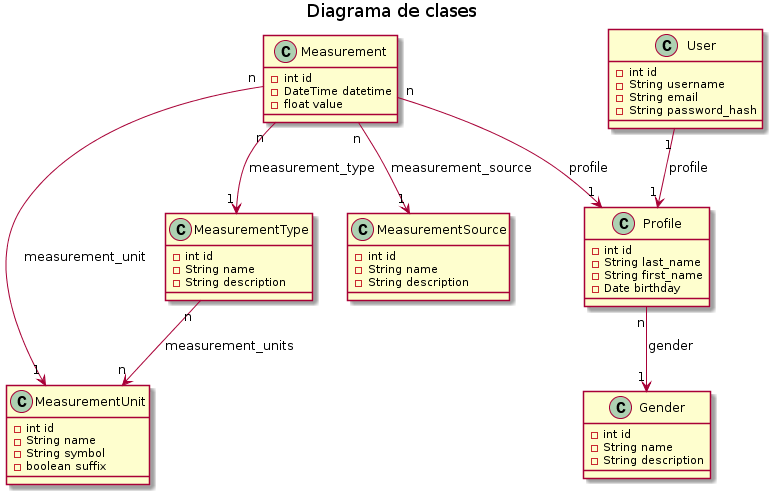
\includegraphics[width=.8\textwidth]{img/3-diagramaClases_relacionTipos}
	\caption{Diagrama de clases donde se puede ver la relación entre el tipo de medición y la unidad}
	\label{relacion_tipo}
\end{figure}


\textbf{ Clase MeasurementType }

Esta clase nos permitirá  nomenclar  los tipos de medidas, hasta el momento hemos contemplado: peso, dimensión corporal (Ej:altura) y glucosa. Existen ciertas medidas que contemplan dos valores, estas serán agregadas en un sprint futuro.

\textbf{Descripción de los atributos}
\begin{itemize}
	\item \textbf{name: }	Nombre del tipo de medición(tipo string).
	\item \textbf{description:} Descripción del tipo de medición (tipo string).
\end{itemize}

\textbf{Dirección del recurso:}
\begin{lstlisting}[language=json,firstnumber=1]
<BASE URL>/measurement_types/{id}
\end{lstlisting}

\textbf{Json generado por la API} 
\begin{lstlisting}[language=json,firstnumber=1]
{
"resource": 
{
"name": "Peso",
"description": "Peso corporal de la persona.",
"id": 1
}
}
\end{lstlisting}

\textbf{ Clase MeasurementUnit }

Esta clase nos permitirá  nomenclar  las unidades de medición disponible para que el usuario pueda seleccionarlas cdo realice la medición, hasta el momento hemos contemplado: Kilogramo, gramo, miligramos, metro, centímetro y milímetro.

\textbf{Descripción de los atributos}
\begin{itemize}
	\item \textbf{id:	}	Identificador único de la unidad de medición(tipo int).
	\item \textbf{name :	}	Nombre de la unidad de medición ( tipo string).
	\item \textbf{symbol :}		Símbolo de la unidad de medición (tipo string).
	\item \textbf{suffix :}	Variable booleana que indica si el símbolo de la unidad de medición es un sufijo (verdadero) o un prefijo (falso) del valor de la medición (tipo boolean).
\end{itemize}

\textbf{Dirección del recurso}
\begin{lstlisting}[language=json,firstnumber=1]
<BASE URL>/measurement_units/{id}
\end{lstlisting}

\textbf{Json generado por la API} 

\begin{lstlisting}[language=json,firstnumber=1]
{
"resource": 
{
"symbol": "Kg",
"suffix": true,
"name": "Kilogramo",
"id": 1
}
}
\end{lstlisting}



Pero fundamentalmente necesitamos el recurso que nos permite traer las unidades de medidas a partir de un tipo particular de medición, dicho recurso se accede por:
\textbf{Dirección del recurso}
\begin{lstlisting}[language=json,firstnumber=1]
<BASE URL>/measurement_types/{id}/units
\end{lstlisting}
\textbf{Json generado por la API} 

Retorna la lista de unidades de medición relacionadas a un tipo de medición específico.
\begin{lstlisting}[language=json, caption=Json generado por la api, label=unitPeso]

{    "resource": 
[{
"id": 1,
"symbol": "Kg",
"suffix": true,
"name": "Kilogramo"
},
{
"id": 6,
"symbol": "g",
"suffix": true,
"name": "gramo"
}]
}
\end{lstlisting}


\subsection{Pruebas ejecutadas}
A continuación se detalla la situación en la que quedaron las pruebas ejecutadas en los sprint anteriores, luego se desarrollarán las soluciones que se usaron y por última se cambiará el estado de aquellas errores encontrados por \textit{"cerrado"}.
        %
	\begin{itemize}
		\item \textbf{¿Qué fue bien?}
        	\begin{itemize}
				\item        Las cargas y ediciones se llevan a cabo correctamente.
			\end{itemize}

   		\item \textbf{¿Qué se mejoró?}
        	\begin{itemize}
				\item \textbf{Cerrado} Al crear una nueva medición, se mostraba un cartel (alert de javascript) con una fecha, dicho alert fue eliminado.
                \item \textbf{Cerrado} Se encontró un problema con la zona horaria que usa el servidor y la zona horaria del usuario, para solucionarlo hubo q hacer un casteo previo cuando se solicitaba la fecha y hora del usuario para mostrar.
			\end{itemize}

   		\item \textbf{¿Qué se puede mejorar?}
        	\begin{itemize}
		        \item \textbf{Abierto} Solo debería mostrarse las unidades relacionadas al tipo de medición que se ha seleccionado 
				\item \textbf{Abierto} En el futuro se deberá mejorar las validaciones de los datos a la hora de cargar información en los formularios.
        		\item \textbf{Abierto} Se deberá mejorar la manera de seleccionar la fecha y la hora. 
                \item \textbf{Abierto} Deberá realizarse los carteles de advertencia necesarios.
            \end{itemize}
       
	\end{itemize}

\textbf{Mostrar unidades relacionadas al tipo de medición seleccionado}

Para evitar errores humanos fue necesario mostrar sólo las unidades de medida que se encuentran relacionadas a un tipo de medición seleccionada por el usuario, por ejemplo: si selecciona Tipo de medición, ``\textit{Peso}'', como se muestra en la \textbf{Figura \ref{unidad_peso}} el sistema solo debería mostrar las unidades que correspondan a ese tipo de medición y no mostrar metros como una posible unidad igual para el caso de que seleccione la altura  \textbf{Figura \ref{unidad_altura}}.

A nivel de frontEnd fue necesario deshabilitar  la selección de unidades cuando el usuario no ha seleccionado el tipo de medición como se indica en la \textbf{Figura \ref{msj_seleccione_tipo}} y una vez seleccionado se tuvo que solicitar a un recurso de la API las unidades relacionadas al tipo de medición seleccionado como se muestran en las figuras antes citadas.

 
 \begin{figure}[h!]
  \centering
  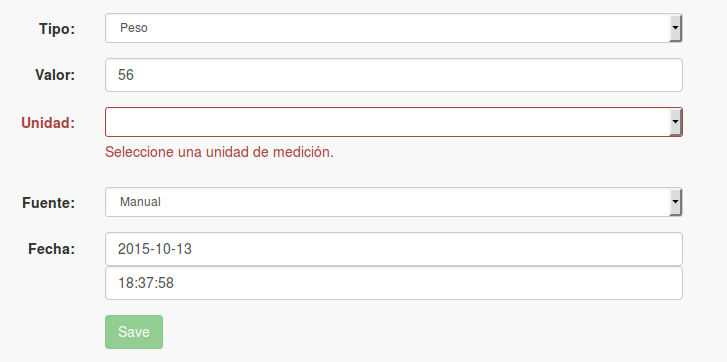
\includegraphics[width=.8\textwidth]{img/3-selecciona_tipo}
  \caption{Mensaje sutil que solicita que se seleccione un tipo de medición }
  \label{msj_seleccione_tipo}
\end{figure}

\begin{figure}[h!]
  \centering
  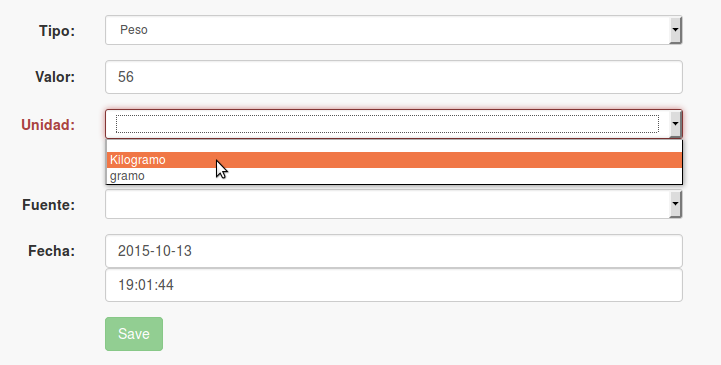
\includegraphics[width=.8\textwidth]{img/3-unidad_peso}
  \caption{Lista de unidades al seleccionar el tipo de unidad ``Peso''}
  \label{unidad_peso}
\end{figure}

 \begin{figure}[h!]
  \centering
  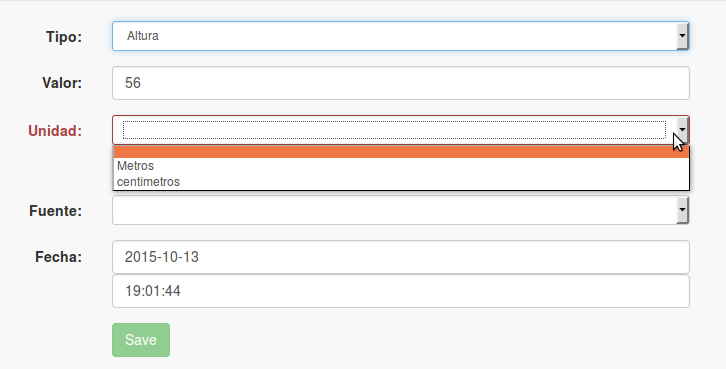
\includegraphics[width=.8\textwidth]{img/3-unidad_altura}
  \caption{Lista de unidades al seleccionar el tipo de unidad ``Altura''}
  \label{unidad_altura}
\end{figure}


El diagrama de clases, las relaciones y los recursos de la API necesarios para poder establecer esta relación se detallan en el apartado \ref{3-clases_involucradas}

\textbf{Carteles de alertas}

Luego de ejecutar las pruebas se detectó que para mejorar la experiencia del usuario es necesario añadir mensajes de avisos, como se muestra en la \textbf{Figura \ref{msj_presiona_no_escribe} y Figura \ref{msj_escribir_borrar}} indicando al usuario situaciones importantes como las que indican ausencia de información importante en el formulario, además el botón para enviar el formulario se mantiene deshabilitado hasta que se haya completado los datos obligatorios (que en este caso serían todos) del formulario.


 \begin{figure}[h!]
  \centering
  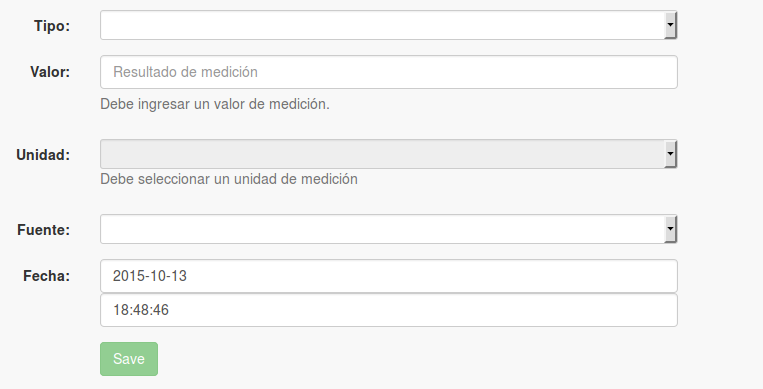
\includegraphics[width=.8\textwidth]{img/3-presiona_no_escribe}
  \caption{Mensaje sutil que aparece  si se ha presionado el campo y no se ha escrito nada}
  \label{msj_presiona_no_escribe}
\end{figure}

\begin{figure}[h!]
  \centering
  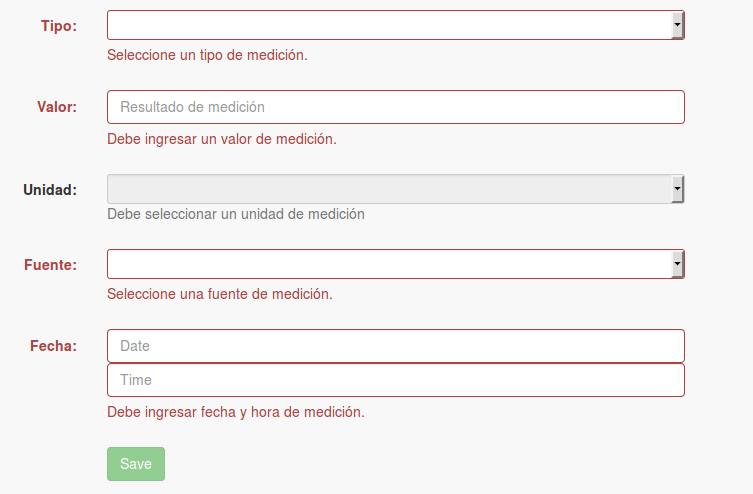
\includegraphics[width=.8\textwidth]{img/3-escribir_borrar}
  \caption{Mensaje vistoso que aparece luego de borrar lo escrito}
  \label{msj_escribir_borrar}
\end{figure}

\clearpage

\begin{lstlisting}[language=JavaScript, caption= recurso que solicita las unidades de un tipo de medición específico, label=type_unit]

 angular.module('saludWebApp')                                                   
 .factory('MeasurementTypeUnit', function (global, $resource) {                  
     // URL of specific API resource                                             
     var url=global.getApiUrl()+'/measurement_types/:id_type/units';             
                                                                                 
     return $resource( url,                                                      
         { id_type: '@_id_type' },                                                        
         { query:{method:'GET',isArray:false},                                   
           update: {method: 'PUT'}                                               
         });                                                                     
}); 
                                                                            
\end{lstlisting}



\textbf{Variable de acceso a la API global}

Fue necesario añadir  un servicio para manejar la dirección global de la API, dicho servicio se detalla en \textbf{Listing \ref{direccion_global}}
\begin{lstlisting}[language=JavaScript, caption= Servicio de la dirección global de la API, label=direccion_global]
'use strict';                                                                   
                                                                                
/**                                                                             
 * @ngdoc service                                                               
 * @name saludWebApp.global                                                     
 * @description                                                                 
 * # global                                                                     
 * Factory in the saludWebApp.                                                  
 */                                                                             
angular.module('saludWebApp')                                                   
  .factory('global', function () {                                              
    // Service logic                                                               
                                                                                
    // URL of yesdoc API                                                           
    var _api_url='https://yesdoc-api.herokuapp.com';                               
                                                                                   
    // Public methods                                                              
    return {                                                                       
      getApiUrl: function () {                                                     
        return _api_url;                                                           
      }                                                                            
    };                                                                             
  });                                                                              
~                                                                            
\end{lstlisting}


\clearpage


\subsection{Estado final de pruebas}

	\begin{itemize}
		\item \textbf{¿Qué fue bien?}
        	\begin{itemize}
				\item        Las cargas y ediciones se llevan a cabo correctamente.
			\end{itemize}

   		\item \textbf{¿Qué se mejoró?}
        	\begin{itemize}
				\item \textbf{Cerrado} Al crear una nueva medición, se mostraba un cartel (alert de javascript) con una fecha, dicho alert fue eliminado.
                \item \textbf{Cerrado} Se encontró un problema con la zona horaria que usa el servidor y la zona horaria del usuario, para solucionarlo hubo q hacer un casteo previo cuando se solicitaba la fecha y hora del usuario para mostrar.
			\end{itemize}

        	\begin{itemize}
		        \item \textbf{Cerrado} Solo debería mostrarse las unidades relacionadas al tipo de medición que se ha seleccionado 
				\item \textbf{Cerrado} En el futuro se deberá mejorar las validaciones de los datos a la hora de cargar información en los formularios.
        		\item \textbf{Cerrado} Se deberá mejorar la manera de seleccionar la fecha y la hora. 
                \item \textbf{Cerrado} Deberá realizarse los carteles de advertencia necesarios.
            \end{itemize}
       
	\end{itemize}